\documentclass[12pt]{article}

\usepackage{packages}
\usepackage{algorithm}
\usepackage{algpseudocode}
\usepackage{amsmath}
\usepackage{tabularx}
\usepackage{graphicx}
\usepackage{subfig}


\graphicspath{{img/}}
\bibliography{sources}
\doublespacing
\graphicspath{{images/}}
\geometry{letterpaper, portrait, includeheadfoot=true, hmargin=1in, vmargin=1in}

%\fontsize{font size}{vertsize (usually 1.2x)}\selectfont

\begin{document}
\renewcommand{\familydefault}{\rmdefault}

\begin{titlepage}
    \begin{center}
    {\fontsize{25}{40}\selectfont \bfseries Industry Project} 
    \\\vspace{15pt}
    {\LARGE Long-Term Portfolio Hedging with Derivatives} \\
    \href{https://github.com/StanPyzhikin/BoA_Berkeley_MFE}{GitHub: Hedging Wealth}

    \vspace{20pt}
    \textbf{} \\
    \textbf{} \\
    \textbf{} \\
    \textbf{} \\
    \textbf{}
    \vspace{8pt}
    % % % % %   IMAGE   % % % % % %
    \vspace{50pt}
    \begin{figure}[h]
        \centering
        
\includegraphics[width=.95\linewidth]{img/UC-Berkeley-Emblem.png}
    \end{figure}
    
    \end{center}
\end{titlepage}
\pagestyle{fancy}
\fancyhf{}
\setlength{\headheight}{0pt}
\renewcommand{\headrulewidth}{0.4pt}
\renewcommand{\footrulewidth}{0.4pt}
\lhead{\large MFE}
\rhead{\large Industry Project}
\rfoot{\textbf{Page \thepage}}
\lfoot{}
\fontsize{11}{13}\selectfont{
\section{Introduction}

\qquad Despite financial markets becoming increasingly efficient, no investor can predict the possibility of a market crash, turbulence, and hold a completely risk-free portfolio. 

Tail-risk refers to the possibility that a crash event affects the portfolio performance significantly. Most hedge fund managers find the use of protective options too costly. They often rely on portfolio diversification rather than derivatives-based hedging to manage tail-risk. Therefore, the motivation of this project is to challenge the statement above and find alternatives involving derivatives.

There are many approaches to implement tail-hedging strategies. Certainly, this topic has gained relevance over the past two decades as the frequency of left-tail events has increased. A simplistic approach may be to buy linear securities that are negatively correlated with the portfolio being held. For example, Treasuries are a good hedge for tail-risk in credit-market crises, especially those at the shortest maturities. However, diversification is not a sufficient tool on its own because the correlations between assets can change under different market regimes. Another approach may be to create a risk-factor model and deliberately take exposures in the risk-factors that are likely to "remove" the portfolio’s negative returns. A popular method involves trend-following strategies which essentially replicate a long position in look-back straddles (long tail-risk). A third approach, the one we explore in this project, requires the purchase of contingent claims. While contingent claims can be a sunk cost to the portfolio if never exercised, options enable an enormous amount of flexibility and can significantly improve the performance of an unhedged strategy in the long-term. 

In this project, we test two approaches empirically: an active put protective monetization strategy by Bhansali [2018] and a European knock-in put option strategy. We also look at other strategies such as volatility index option strategies as a reference point. We compare the three approaches using Sharpe, drawdown and net returns over 21 years. We concluded that active monetization and European knock-in options have better results than volatility-index hedging (VIX calls for example), but come at the cost of liquidity and transaction costs which are difficult to measure. We provide a careful and active monetization strategy that performs well despite liquidity constraints and transaction costs. We conclude the same as (Bhansali, 2014), a well-monitored active monetization strategy can not only hedge the downside of a portfolio but also turn it into an offensive tail-risk hedging strategy in the medium-term.


\pagebreak
\tableofcontents
\pagebreak

% % % % % % % % % % % % % % % % % % % %
% % % % %  REPORT CONTENT   % % % % % %
% % % % % % % % % % % % % % % % % % % %

\fontsize{11}{15}\selectfont{

\section{Literature Review}

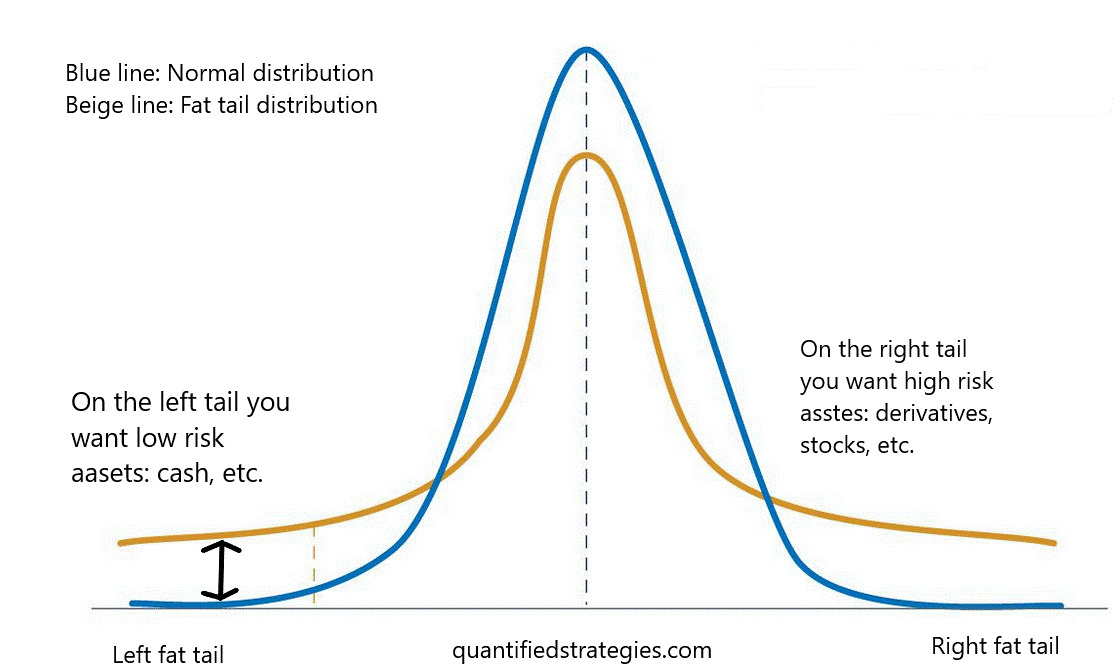
\includegraphics[width=\textwidth]{cufvef.jpeg}

\qquad In order to avoid repetition of work, it is important to explore and summarise the key strategies and results of previous academics in this field. We will often refer to work by Bhansal and Israelov, who are industry experts with several papers, among others throughout this project. 

Bhansali is the founder of LongTail Alpha, a hedge fund with an expertise in tail-risk management. He has published several papers such as ‘Monetization Matters: Active Tail Risk Management and the Great Virus Crisis, 2020’, ‘Right Tail hedging: Managing Risk When Markets Melt Up, 2018’, ‘Tail-risk management for retirement investments, 2015’ and has a book called ‘Tail-Risk Hedging: creating robust portfolios for volatile markets, 2013’. Bhansali claims that tail-risk management strategies are a ‘necessity, not a luxury’ and his paper on active tail risk management sets a rubric to manage the purchase of protective puts to optimise their net value to the portfolio. 

Roni Israelov serves as Chief Investment Officer and President at NDVR. NDVR provides quantitative wealth management tools and advisory. His past papers often offer a conflicting view to Bhansali’s on derivatives based hedging strategies for tail-risk management. Israelov and Nielsen [2015] empirically investigated whether put options purchases make economic sense especially in periods when equity volatility is low and they may appear to be cheap. He concludes that this is an illusion and that buying puts, in expectation, leads to losses for many years. ‘We believe the frequency of black swan events required to rationalise option purchases is unreasonably large’. 

Therefore, we will be empirically testing the claims by Bhansali vs Israelov and conclude whether there is indeed economical value in a protective put strategy. Before we dive deeper into Bhansali’s work and outline the methodology in his paper, let’s take a look at other frameworks and literature. 
	
\qquad Another paper that covers using put options as a hedging instrument is the article "Warren Buffett versus Zvi Bodie: Should you buy or sell put options?" by Steen Koekebakker and Valeriy Zakamulin. It covers two views of using put options in clients’ portfolios: buying and selling. The article delves into Warren Buffett and Zvi Bodie's contrasting opinions on buying or selling long-term put options. Bodie argues that the cost of insuring a portfolio at expiration is inexpensive for long-term horizons and he recommends it to every portfolio manager. On the other hand, Warren Buffett argues that long-term portfolio insurance is expensive and does not pay off. He supports his arguments with a numerical example. 

\qquad The authors then delve into the scientific studies that have examined the optimality of portfolio insurance on empirical and theoretical grounds. They discuss the works of Jacobs (1983), Haugh and Lo (2001), Driessen and Maenhout (2007), and Døskeland and Nordahl (2008), among others. The authors conclude that previous research presents little support for the optimality of portfolio insurance.

\qquad The authors use the method of mean-variance optimization to maximize the bi-linear utility function, which describes risk-averse investors. One essential finding is that when the investment horizon approaches infinity, the stock market risk vanishes if the expected stock market return exceeds some threshold. Specifically, when $\mu > \kappa +0.5\sigma^2 + 2\sigma\sqrt{\kappa}$. Otherwise, the stock market risk increases to infinity. For example, if $\kappa = 0$ and $\sigma = 20\%$  (this is the average U.S. stock market volatility), then the stock market risk vanishes in the long run for all $\mu>2\%$ , which is significantly lower than the average US market stocks return.

\qquad In conclusion, the authors find that when the investment horizon is short, it is optimal to buy put options. However, when the investment horizon increases, it is optimal to sell put options. As our project is focused on mid-term investments: 3-5 years, it can be concluded that using puts as a hedge is an appropriate strategy for risk-averse investors, as in accordance with the article, the stock’s riskiness increases in the short run. And risk attains a maximum at approximately 3.3 years. 

\section{Methodology}

\subsection{Strategy 1: Active Monetization of Vanilla Protective Puts}

\qquad While it is true that puts can be used as a hedge, they can be expensive and create a significant drawdown to the portfolio. Bhansali argues that most researchers have not paid enough attention to the consequential impact of active management of their tail hedging portfolio. Having a passive approach is indeed extremely costly and inefficient, however through simple monetization rules, Bhansali found that in the medium to long term horizon (3+ years), cumulative returns on an active put strategy net significantly higher than a passive strategy. In fact, over the period from 1950 to 2009, cumulative returns on an actively managed put portfolio net to about a 30 percent gain over an unhedged S\&P500 position. Moreover, a passive put portfolio nets to about a 16 percent loss over an unhedged S\&P500 position (Bhansali, 2014). We aim to validate these numbers. 

\subsubsection{Rules}
Based on Bhansali(2020)'s work, we replicated an active strategy backtested from 2000 to 2021 with the following rules:

\begin{itemize}
  \item Allocate 3\% of our portfolio annually to the purchase of OTM put options. Experiment with options of varying maturities, ranging from short-term (3 months) to medium-term (1 year) options. It is important to note that the rebalance period is the same to the maturity of the put options that we use.
  \item Define monetization thresholds (2.5x, 5.0x, 7.5x). If the value of the put option exceeds the purchase value by the monetization threshold, an exit strategy is initiated. Otherwise, the option is held until expiration.
  \item Define exit values for put options (0.5, 1). This parameter determines whether we sell the entire put option or only sell a portion and keep 50\% of the option position when the monetization threshold is reached.
\end{itemize}

Similar to Bhansali (2020), we used the Black-Scholes parametric model (including dividends) (\ref{firsteqn}) to relate the prices of options at different strikes and maturities to the market environment. In our results, we also simulate one approach using real historical prices (Eriksson and Bendiksby, 2021).

\begin{equation}\label{firsteqn}
P = Ke^{-rT}\phi(-d2) - Se^{-yT}\phi(-d1)
\end{equation}
\begin{math}
\begin{multiline}
d1 = (log(S / K) + (r - y + (sigma ** 2) / 2) * T) / (sigma * sqrt(T)) \\
d2 = d1 - sigma * sqrt(T)
\end{multiline}
\end{math} \\




We begin with a portfolio of \$10,000, with \$9,700 allocated to the purchase of S\&P500 on day one, and \$300 allocated to the purchase of OTM put options (10-30\% OTM). We calculate a target price based on the stock: option cash allocation ratio and the underlying spot price:

\begin{equation}
TargetOptionPrice_{t} = SP500price_{t-1} * (OptionCashAllocation)/(SP500CashAllocation)
\end{equation}

The strike price is then found through Black-Scholes. As a benchmark, this is expected to be in the 10-30\% OTM range. 

\textbf{Transaction Costs}
In order to make the performance realistic, we had to account for transaction costs for each of our option and underlying purhcases. We used a constant value of 4.9bps as the transaction cost as per industry standard (Bhansali, 2014 and Erikkson, 2021). We note that incorrectly valued transaction costs can impose a significant impact on performance. Hence, we choose a high figure to be conservative. 

\subsubsection{Exit Strategies}
\qquad Once a purchased put option reaches its monetization target, Bhansali(2014) would sell the option and purchase a new option on the same date. The difference between the sale and repurchase of a further OTM put option was kept in cash. In our project, we explore additional strategies such as:
\begin{itemize}
\item 1. Equity Reinvestment: Proceeds from the option sale are used to reinvest in the underlying.
\item 2. Partial Monetization: A fraction of the option is sold while the rest is kept until expiration.
\item 3. Early Monetization with no Repurchase: Once an option is sold early, we remain unhedged until the original expiration date of the option, when we purchase the next option. 
\end{itemize}
\qquad To implement the above strategies, we have defined two types of monetization strategies, each with variations in parameters:
\begin{itemize}
\item M1: Once our purchased put options reach their monetization target, we either sell 50\% (partial monetization) or 100\% (complete monetization) of the option. The proceeds are then reinvested in equity. We refrain from purchasing a new put option until the next rebalancing period.

\item M2: When our purchased put options reach the monetization target, we sell the entire option (complete monetization). We reinvest 50\% or 100\% of the proceeds in new put options with the same maturity date, maintaining the hedge ratio unchanged. The difference between the sale and purchase amounts of the option is reinvested in equity.

\end{itemize}
\qquad For each of the above monetization strategies (M1 and M2), we tested different parameters to evaluate their effectiveness in achieving our objectives.

\subsection{Strategy 2: European Knock-In Put Options}

\qquad Put options can be used as a hedge on a mid-term horizon. This results in two main selections that need to be addressed: parameters of put options and weights of options in a portfolio. Hedging with vanilla ATM puts is efficient; however, it can be expensive and significantly affect the performance of a portfolio. In this project, we tested the hypothesis that using exotic options for hedging purposes may be beneficial.

\qquad Barrier options can be used as an alternative to vanilla put options; the main advantage of barrier options is their price. Adding a barrier decreases the option's price, but investors usually face the tradeoff between a low price and an efficient hedge. When trying to minimize the option premium, we run the risk of setting the barrier too low. In this case, the probability of execution decreases. On the other hand, moving a barrier to the strike on the upper bound, we have a vanilla ATM put option. In this case, the option will be executed more often at the expense of a higher premium.

\qquad In this project, we will use European knock-in put options with barriers below the current strike level. The solution for these options can be found in closed form. For this, we need to make same assumptions regarding the Black-Scholes model. We assume that stocks have Log-normal dynamics, constant volatility, and constant interest rate. 

\begin{equation}
\begin{aligned}
\text{Knock-In Put} &= -\text{S} \times \Phi (-\text{d1}) + \text{S} \times e^{-\text{r} \times \text{T}} \times \Phi(-\text{d2}) \\
&\quad + \text{S} \times \left(\frac{\text{B}}{\text{S}}\right)^{\frac{2 \times (\text{r} + \sigma^2)}{\sigma^2}} \times \left(\Phi(\text{d3}) - \Phi(\text{d1})\right) \\
&\quad - \text{S} \times e^{-\text{r} \times \text{T}} \times \left(\frac{\text{B}}{\text{S}}\right)^{\frac{2 \times \text{r}}{\sigma^2}} \times \left(\Phi(\text{d4}) - \Phi(\text{d2})\right)
\end{aligned}
\end{equation}

Where:
\begin{align*}
\text{d1} &= \frac{\ln\left(\frac{\text{S}}{\text{K}}\right) + \left(\text{r} + \frac{1}{2} \times \sigma^2\right) \times \text{T}}{\sigma \times \sqrt{\text{T}}} \\
\text{d2} &= \text{d1} - \sigma \times \sqrt{\text{T}} \\
\text{d3} &= \frac{\ln\left(\frac{\text{S}}{\text{B}}\right) + \left(\text{r} + \frac{1}{2} \times \sigma^2\right) \times \text{T}}{\sigma \times \sqrt{\text{T}}} \\
\text{d4} &= \text{d3} - \sigma \times \sqrt{\text{T}}
\end{align*}
\qquad Where:

\qquad r = Interest rate, \quad S = Spot, \quad K = Strike, \quad B = Knock In Barrier, \quad $\sigma$  = Volatility, \quad T = Time to expiration, \quad $\Phi$ = CDF of Normal Distribution

\subsubsection{Weight optimization using a mean-variance framework}

\qquad To address the issue of optimal option weights, we will use mean-variance optimization. As a proxy for the US stock market, we will take the SPX index. This way, the portfolio will contain the SPX index and put/knock-in put options. 
\begin{align*}
\text{Log returns} = \ln\left(\frac{\text{Close price (t)}}{\text{Close price (t-1)}}\right) \
\end{align*}
\begin{algorithm}
\caption{Calculate mean returns and covariance matrix}
\begin{algorithmic}[1]
\State $\text{Mean returns} \gets \text{Log returns/n}$
\State $\text{Covariance matrix} \gets \text{Log returns}$
\end{algorithmic}
\end{algorithm}
\begin{align*}
\text{Return} &= \sum_{i=1}^{n} \text{Mean returns}_i \times \text{weights}_i \times 252 \\
\text{Portfolio Std} &= \sqrt{\text{weights}^T \cdot \text{Covariance matrix} \cdot \text{weights}} \times \sqrt{252}
\end{align*}


The Sequential Least Squares Programming (SLSQP) method is used to solve the following optimization problem:

\begin{algorithm}
\caption{Sequential Least Squares Programming (SLSQP) Method}
\begin{algorithmic}[2]
\State Initialize $x$, the solution vector
\While{not converged}
    \State Compute the gradient of the objective function $f$, $\nabla f(x)$
    \State Solve the quadratic programming subproblem to get a direction of search, $p$
    \State Line search: Find an optimal step size, $\alpha$, that minimizes $f(x + \alpha p)$
    \State Update the solution vector, $x \gets x + \alpha p$
\EndWhile
\State \Return $x$
\end{algorithmic}
\end{algorithm}

\qquad Using the methodology described above, we are getting the optimal weights of tge portfolio consisting of the S\&P 500 index and the hedging component.

\subsection{Data Sources}

\qquad We used the Python Yahoo Finance API to retrieve the majority of the underlying stock data. This provides a convenient and efficient way to access financial data for a broad range of financial instruments including stocks, commodities, and currencies. Here are several reasons in favor of the selection of this data source:

\begin{enumerate}
\item \textbf{Wide Coverage}: The Yahoo Finance API covers a broad range of global financial instruments including stocks, ETFs, mutual funds, futures, options, commodities, currencies, and more.
\item \textbf{Historical Data}: The API provides historical market data, going back many years for many securities, allowing for thorough backtesting and analysis.
\item \textbf{Real-Time Data}: Although limited, the API provides some real-time data, which can be critical for short-term trading strategies.
\item \textbf{Additional Financial Data:} Besides price data, Yahoo Finance offers other financial data such as: financial statements, dividends, stock splits, and even some analyst estimates, which can be useful for a more in-depth analysis.
\item \textbf{Ease of Use}: The API is simple to use, especially with Python libraries like yfinance or pandas-datareader that provide easy-to-use functions to access the data.
\item \textbf{Free of Charge}: Perhaps one of the most attractive features is that all of this data is available for free. While there are some limitations in terms of the amount of requests one can send, for many individual users, these limitations are sufficient.
\end{enumerate}

\qquad To estimate the price of the options we need several parameters: strike, spot, interest rate, volatility, and time to expiration. The most controversial parameter is volatility. The Black-Scholes method assumes constant volatility which doesn't hold due to the "volatility smile". This means that if we go far out-of-the-money, volatility often tends to increase. However, we neglect the "volatility smile" effects as we are primarily focused on the area around the strikes. As a proxy of volatility, we decided to use the VIX.
\qquad The VIX, or Volatility Index, often referred to as the "fear index", is a real-time market index representing the market's expectations for volatility over the coming 30 days. It is calculated and published by the Chicago Board Options Exchange (CBOE). Also, it is derived from the prices of a basket of S\&P500 index options.

\qquad The calculation of the VIX is a bit complex, but it can be described in general terms as follows:

\[
VIX = 100 \sqrt{(2K \times \frac{\sum Q(K) e^{RT} \Delta K}{S_0}) - \frac{1}{T}\left(\frac{F}{S_0} - 1\right)^2}
\]

where:
\begin{itemize}
\item $K$ is the strike price of the S\&P500 index option,
\item $Q(K)$ is the midpoint of the bid-ask spread for each option with strike $K$,
\item $T$ is the time to expiration,
\item $R$ is the risk-free interest rate,
\item $F$ is the forward index level, and
\item $S_0$ is the current level of the S\&P500 index.
\end{itemize}

This formula sums the squared prices of put and call options and applies a series of weights.

\textbf{Historical Options Prices for VIX and the S\&P500}

We used the IvyDB from OptionsMetrics for our historical option price datasets. We collected data of European SPX puts and VIX calls, which we then filtered for deltas to suit our OTM range. This was only looked at in the improvement section of this paper. In particular, we address the assumptions of using Black-Scholes implied prices for our report and recognize this as a potential area of improvement.

\textbf{Risk-free rate}

We took Treasury's 3-month T-bill rate (DTB3) which we retrieved using the FRED API. This was used as an input to Black-Scholes and to calculate excess returns (and Sharpe ratios). 

\subsection{Metrics: Sharpe Ratio, Max Drawdown, Portfolio Return}

\qquad One of the critical topics in similar research is choosing the appropriate metrics to evaluate the efficiency of the applied method. In this paper, we decided to use 3 main metrics: Sharpe ratio as a metric of risk-reward, maximum drawdown as a metric of downside risk, and portfolio return as a metric of return/profitability. 

\textbf{Sharpe Ratio}

The Sharpe Ratio is a widely used financial metric that helps investors understand the return on investment compared to its risk (risk-adjusted metric). It is the average return earned in excess of the risk-free rate per unit of volatility or total risk. The Sharpe Ratio can be calculated as follows:

\[
\text{Sharpe Ratio} = \frac{R_p - R_f}{\sigma_p}
\]

Where:
\begin{itemize}
\item $R_p$ is the expected portfolio return,
\item $R_f$ is the risk-free rate, and
\item $\sigma_p$ is the standard deviation of the portfolio's excess return.
\end{itemize}

\qquad The Sharpe Ratio is beneficial because it adjusts for risk, allowing for a direct comparison of investment options irrespective of their risk profiles. A higher Sharpe Ratio indicates a more attractive risk-adjusted return, making it a good metric for performance estimation.

\textbf{Max Drawdown}

In this paper, we define the maximum drawdown as the largest decline in an investment's value, expressed as a percentage, measured from a peak to the subsequent trough.

We wrote a function in Python to calculate this metric. It takes the time series of returns of our strategy as input, computes the cumulative returns and then runs through each time step storing the percentage decline between the cumulative returns and the previous peak. It then outputs the maximum value of these stored drawdown values.

\textbf{Other Metrics}

Some other tail-risk standard metrics we could have looked at are expected shortfall (Homescu, 2014) and parametric-VaR (Bhansali, 2014). However, to keep benchmarks simple for any user to comprehend and calculate, we used the three metrics mentioned.

\subsection{Other Strategies: VIX options, OTC Variance Swaps}

\qquad Other than protective puts or knock-in puts on the underlying, some investors look at volatility hedging as a tool for managing the tail-risk in their portfolios. According to Szado (2019), "meaningful portfolio diversification benefits for risk-averse investors are possible over particular time periods with small allocations to long VIX futures or call options, but there can be substantial portfolio drag if large allocations are made over long time periods during which there are flat to rising stock markets". 

Therefore, to further improve our analysis on protective puts, we decided to have a rough benchmark for a volatility hedging strategy to compare to. We proceeded with a strategy to purchase 25\% OTM monthly calls on VIX on a monthly basis (taking them to expiry and repurchasing every month). We tested this over a smaller sample period of 2006 to 2021 due to the lack of VIX data. 

One area of investigation in this field is dynamic allocation to VIX calls which we may be interested in for a future paper. One can analyse market regimes and come up with rules on when/how to allocate these calls. Holding VIX calls monthly over 2008 and 2020 proved to be extremely lucrative, but over the long-term during bull markets it doesn't seem to perform well. 

There are many other tools for hedging that we could also look at. Examples include OTC variance swaps that allow one to speculate on or hedge risks associated with the volatility of your underlying. In a variance swap, two parties enter a contract on forward realized variance. At maturity it pays the difference between the realized variance and the agreed variance strike.

However, the reason we decided to pursue an improvement to put option strategies is due to the evidence in literature that simple volatility index option strategies seem to have a large drawdown in the long term. On the other hand, Bhansali has suggested this may not be the case with actively monetized puts and collars directly on the underlying stock.

\section{Results}
In this section, we compare the key performance metrics of the strategies mentioned vs a benchmark portfolio of S\&P500. The key takeaway from our empirical studies is that active monetization strategies considerably reduce max drawdown (roughly 13\%) and also increase Sharpe (61\%) over the medium-term. Knock-in options (which use a barrier to provide more control over the payout) are also successful at reducing drawdown (15\%). However it is important to recognise the illiquidity of this type exotic instruments. Lastly, in our empirical studies, an alternative simple VIX option strategy performed much worse with a very small increase in Sharpe and reduction in drawdown. Figure 1 below summarises this. 

\begin{figure}[htp]
    \centering
    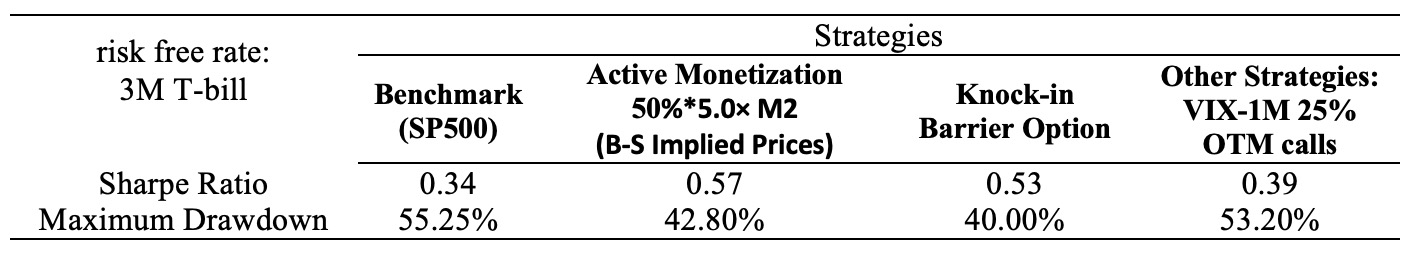
\includegraphics[width=15cm, height=2.5cm]{summary.jpg}
    \caption{Performance comparison on 21 year time frame}
    \label{fig:galaxy}
\end{figure}



\textbf{Caveats: what defines mid-term?}

While we haven't investigated the short-term, several papers (Doran, 2020 or Bhansali, 2016) have concluded that tail-risk hedging with options doesn't work in the short-run due to the transaction costs and low probablity of a tail-event occuring in the short-run. As we extended the previous case study figures of Bhansali, by also incorporating 2018, 2019 and 2020 to capture a period over 21 years, it is important to question what length or time period is sufficiently worth it for a tail-risk strategy. 

Let's take a deeper look at the two strategies:

\subsection{Active Monetization of Protective Puts}
\qquad In this section, we will begin by using the B-S (Black-Scholes) implied prices to assess the overall impact of monetization from 2000 to 2021. Following that, we will analyze its performance during historical left and right-tail events. To ensure the reliability of our findings, we conducted tests on real OptionsMetrics option prices and trade information using one of the strategies mentioned earlier.

\textbf{B-S Implied Prices}

The Figure2 below presents three relevant variables for these charts. First, the "monetization threshold" is defined as the multiple of the initial option value at which monetization occurs. For instance, "5.0x" implies monetization takes place when the options' value reaches or exceeds five times their original price. Second, we specify the extent of monetization and the use of proceeds. In the attached charts, we consider 50\% or 100\% monetization, with distinct implications for two monetization strategies. For M1, we assume 50\% or 100\% of the positions are liquidated when the monetization threshold is reached, and the cash is reinvested in the stock. For M2, we liquidate the entire position once the threshold is hit but use 50\% or 100\% of the cash to repurchase put options to maintain the hedging ratio, while the remaining cash is used to buy stock. Last, we define the rebalancing period. For instance, if we rebalance annually, we need to buy put options with a maturity equal to one year. If we monetize before their maturity and repurchase new put options, the new put options must have the same maturity date as the prior ones.

\begin{figure}[htp]
    \centering
    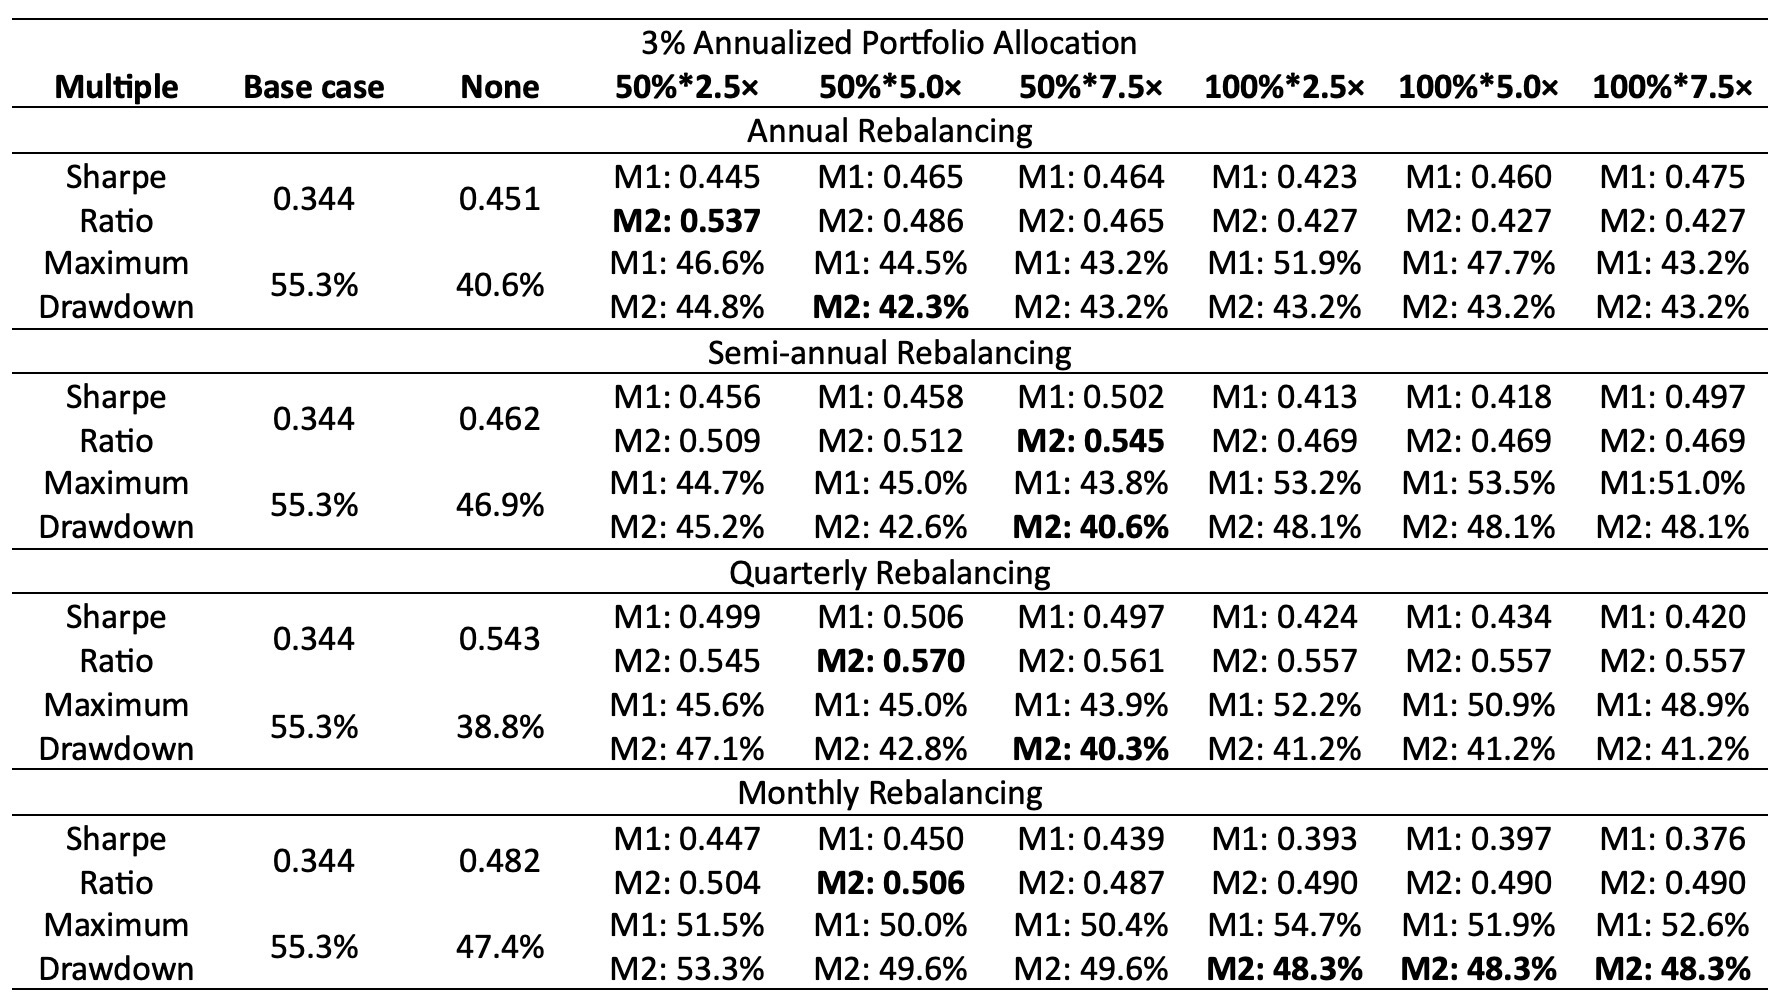
\includegraphics[width=14cm]{results.jpg}
    \caption{Performance Comparison of Active Monetization Over a 21-Year Time Frame}
    \label{fig:galaxy}
\end{figure}

When comparing the base case and the no-monetization line with various monetization strategies, it becomes evident that adopting monetization strategies leads to improved Sharpe ratios compared to the no-monetization approach, while still maintaining a satisfactory level of hedging protection indicated by the max drawdown. This is especially noticeable for the partial M2 monetization strategy with lower multiples and lower rebalancing frequency.

To closely examine the performance during specific tail risk events, we selected two typical left tail risk events and two right tail risk events. Based on the figures below, we observed that during the Global Financial Crisis (GFC) and the COVID-19 crisis, the monetization strategy effectively hedged against left tail risk. It significantly reduced the maximum drawdown compared to the unhedged base case. Conversely, during the post-GFC period of 2011-2014 and the pre-COVID period of 2016-2019, when the stock market performed well with right tail cases, the monetization strategy improved performance compared to the traditional holding-to-maturity put strategy.

Both findings align with those of Bhansali (2014), suggesting that a well-monitored active monetization strategy can not only provide downside protection to a portfolio but also act as an offensive tail-risk hedging strategy in the medium-term.

\begin{figure}[htp]
    \centering
    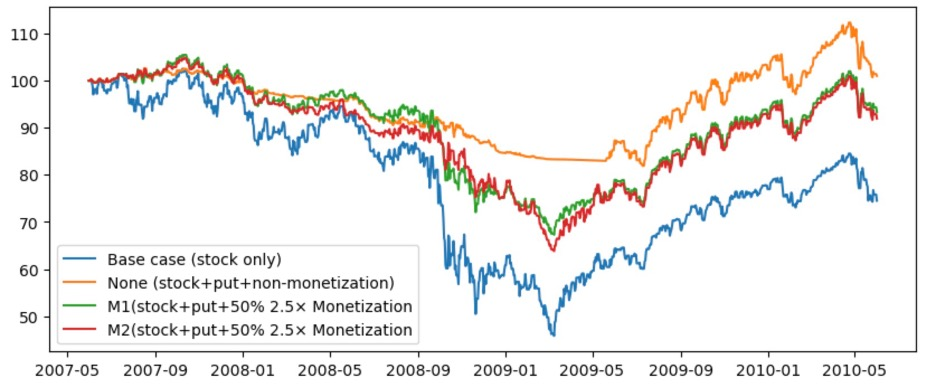
\includegraphics[width=14cm]{left_tail_event1.jpg}
    \caption{Impact of partial monetization left tail hedging strategy during the GFC of 2008-2009}
    \label{fig:galaxy}
\end{figure}

\begin{figure}[htp]
    \centering
    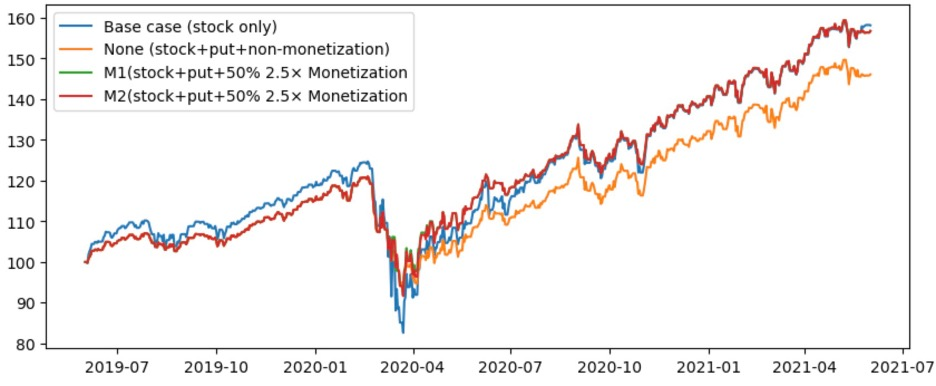
\includegraphics[width=14cm]{left_tail_event2.jpg}
    \caption{Impact of partial monetization left tail hedging strategy during the COVID-19 crisis in Q2 of 2020}
    \label{fig:galaxy}
\end{figure}

\begin{figure}[htp]
    \centering
    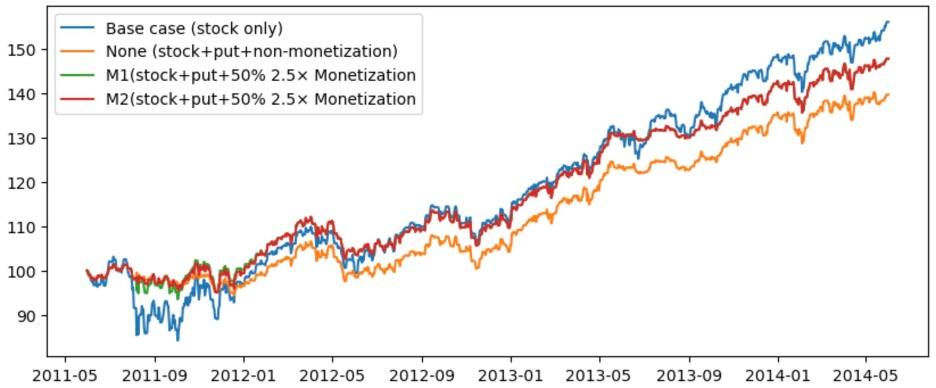
\includegraphics[width=14cm]{right_tail_event1.jpg}
    \caption{Impact of partial monetization of right tail hedging strategy during the post GFC period of 2011-2014}
    \label{fig:galaxy}
\end{figure}

\begin{figure}[htp]
    \centering
    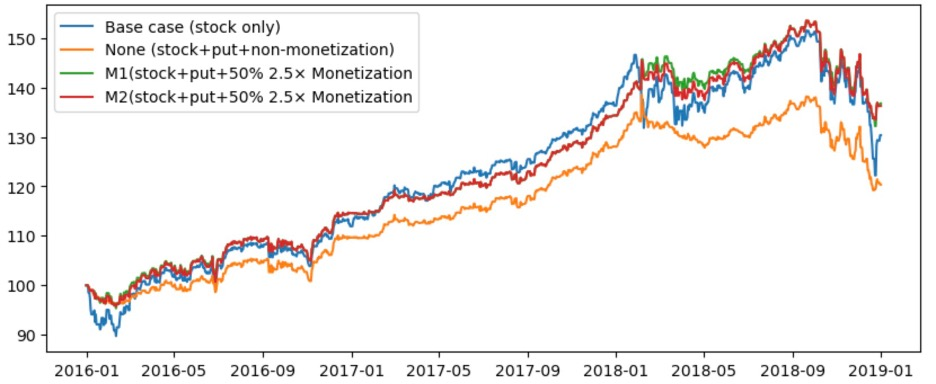
\includegraphics[width=14cm]{right_tail_event2.jpg}
    \caption{Impact of partial monetization of right tail hedging strategy during the pre-COVID period of 2016-2019}
    \label{fig:galaxy}
\end{figure}

\textbf{Historic Option Prices}
While the results above look promising, one of the underlying assumptions we made was on finding liquid options at the prices we expect. To test robustness, we ran one of the strategies above on real OptionsMetrics option prices and trade information. 

We ran the 100\%*2.5x quarterly rebalancing strategy. While we assumed above that it was easy to rebalance with options maturing in a quarter, in reality there were some trade dates with no quarter maturity options meeting the required moneyness constraints. Hence, for specific trade date cases such as this, we tried shorter maturities of 1 and 2 months instead - leading to more rebalancing.

Overall, the strategy had a similar performance with a slight decrease in sharpe due to lower excess returns. This was partially due to an increase in transaction costs from the additional rebalancing required due to liquidity. The Sharpe and Max Drawdown are compared to the previous values using Black-Scholes in figure 6 below.

\begin{figure}[htp]
    \centering
    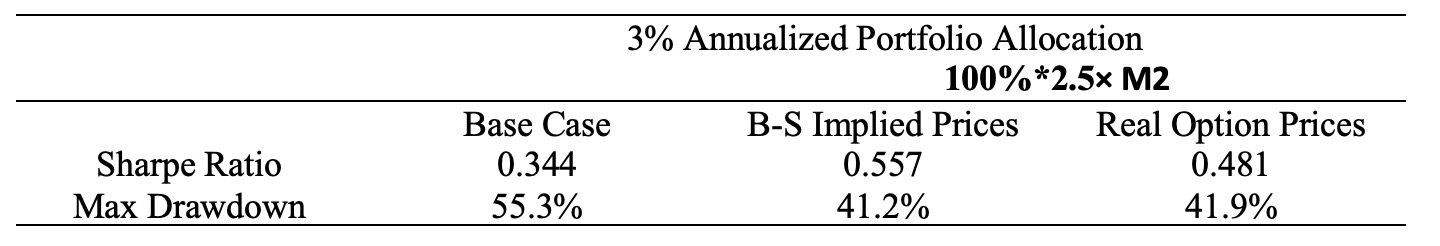
\includegraphics[width=14cm]
    {compare.jpg}
    \caption{Running a specific 100\% active monetization at a 2.5 multiple scenario with real options prices. Comparing results using real options prices vs BS-implied options prices.}
    \label{fig:galaxy}
\end{figure}

\subsection{Knock-In Put Hedging Strategy}

\qquad Once we have obtained all required data and methodology, we can implement it in practice. Using mean variance optimization method we calculate optimal weights of hedge in portfolio. We assume all put and knock-in put options have six month maturity. Vanilla put option are ATM, for knock-in put options barrier is 95\%. As risk free rate we use annualized 3 month Treasury bills. In the table below you can see, that optimal weight of investment in hedging is around 2.5\% for vanilla put options, which approximately corresponds to 62.5\% coverage of SPX part. For knock-in options weight is approximately 3\% which corresponds to 95\% coverage. This can be explained by the fact, that knock-in options are on average 18\% cheaper than vanilla put options.\\

\begin{tabularx}{0.7\textwidth} { 
  | >{\raggedright\arraybackslash}X
  | >{\raggedright\arraybackslash}X 
  | >{\raggedright\arraybackslash}X |
 }
 \hline
 \textbf{Weights} & \textbf{SPX}  & \textbf{Hedge}  \\
 \hline
 \textbf{SPX+Put} & 97.563\%  & 2.437\%   \\
 \hline
 \textbf{SPX + KI Put} & 97.056\%  & 2.944\%   \\
 \hline
\end{tabularx}
\\

\qquad Despite the fact, that in article of Teen Koekebakker and Valeriy Zakamulin was mentioned, that on a long horizon risk averse investors will be likely selling options, to compare this strategy with other we tested it on 20 years horizon, starting from 2000 to 2020. At Figure 1, we show the performance of three strategies: pure long SPX, long SPX + heding using vanilla put options, long SPX + hedging using knock-in put options. As can be see from the metrics: both strategies with hedging show better Sharpe ratio at the same time with smaller maximum draw down. Average return of hedging strategies is smaller than pure long strategy, but only by 0.1\% per year. \\

\begin{figure}[htp]
    \centering
    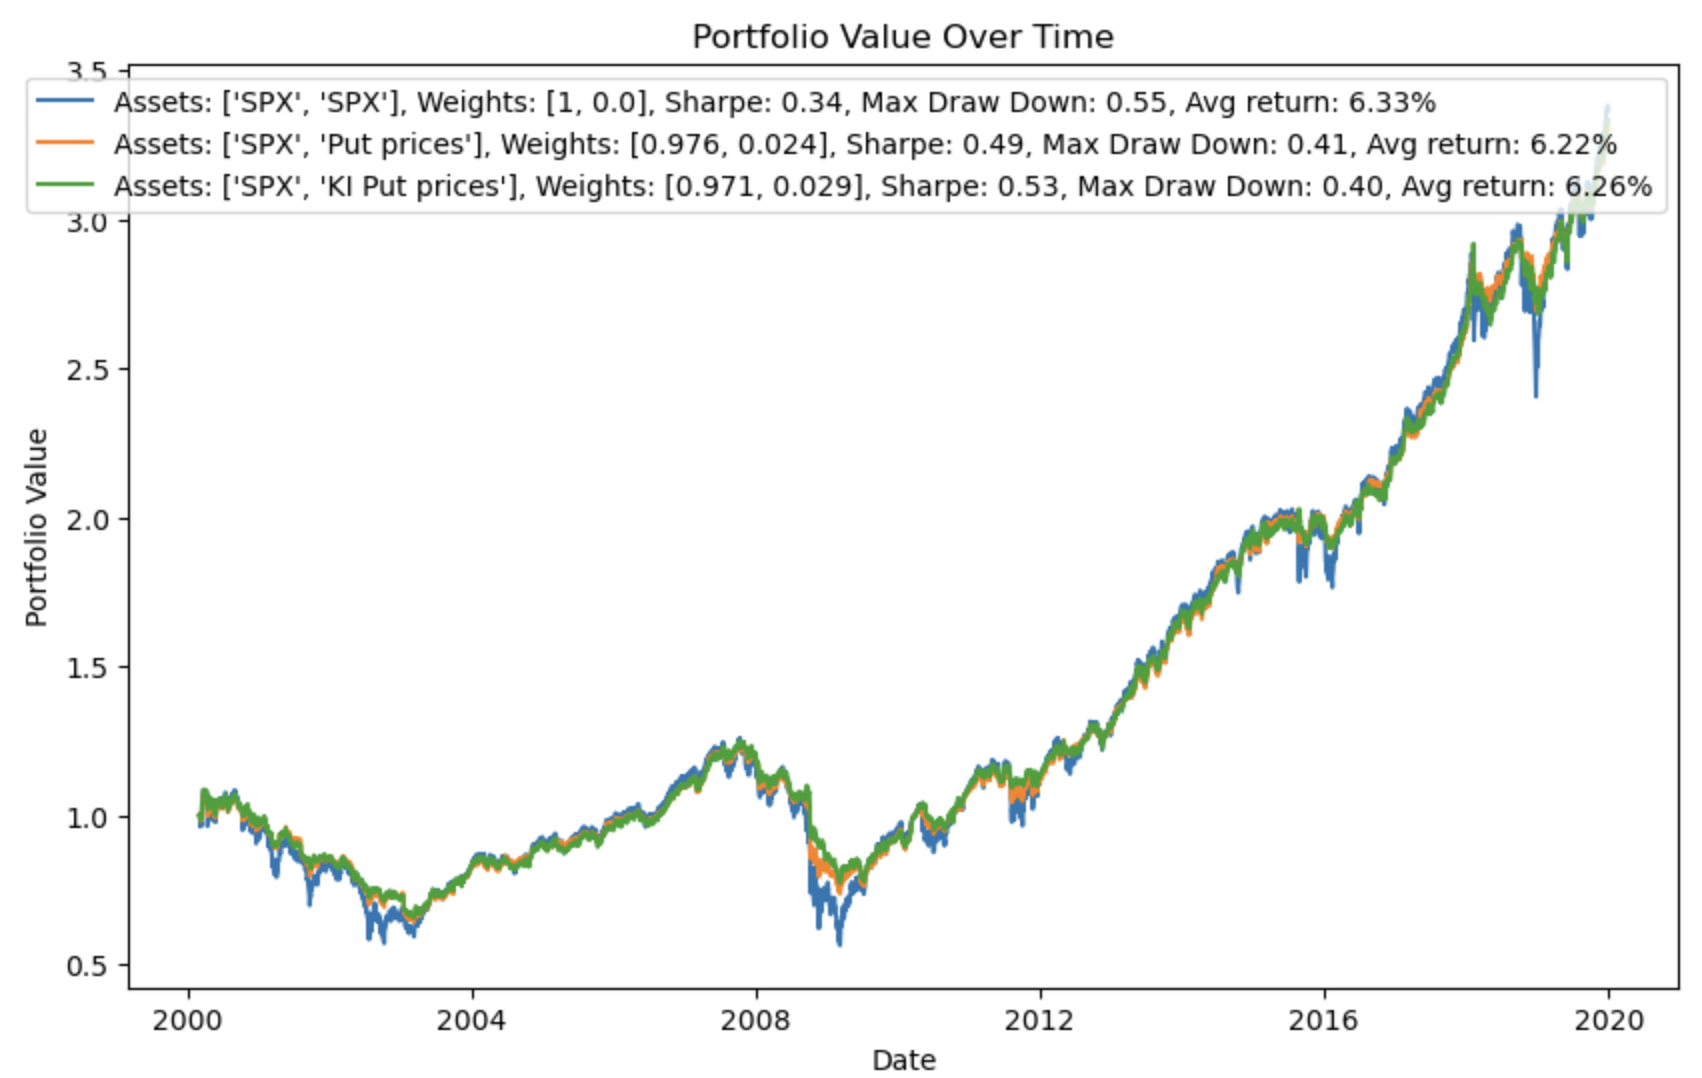
\includegraphics[width=14cm]{20years.png}
    \caption{Performance comparison on 20 year time frame}
    \label{fig:galaxy}
\end{figure}

\qquad Our main hypothesis for this strategy was that it will be more efficient on mid-term horizon. We tested this using 5 year rolling window. Starting from 2001-01-03 each day we run all strategies and obtained the Sharpe ratio, average return and max draw down. We ran these strategies for 10 years, which covers both growing and falling market conditions. On the graph below, we can see, that the Sharpe ratio of hedging strategies is higher than pure long, as expected. However, results between vanilla put and knock-in options are ambiguous.  \\

\begin{figure}[htp]
    \centering
    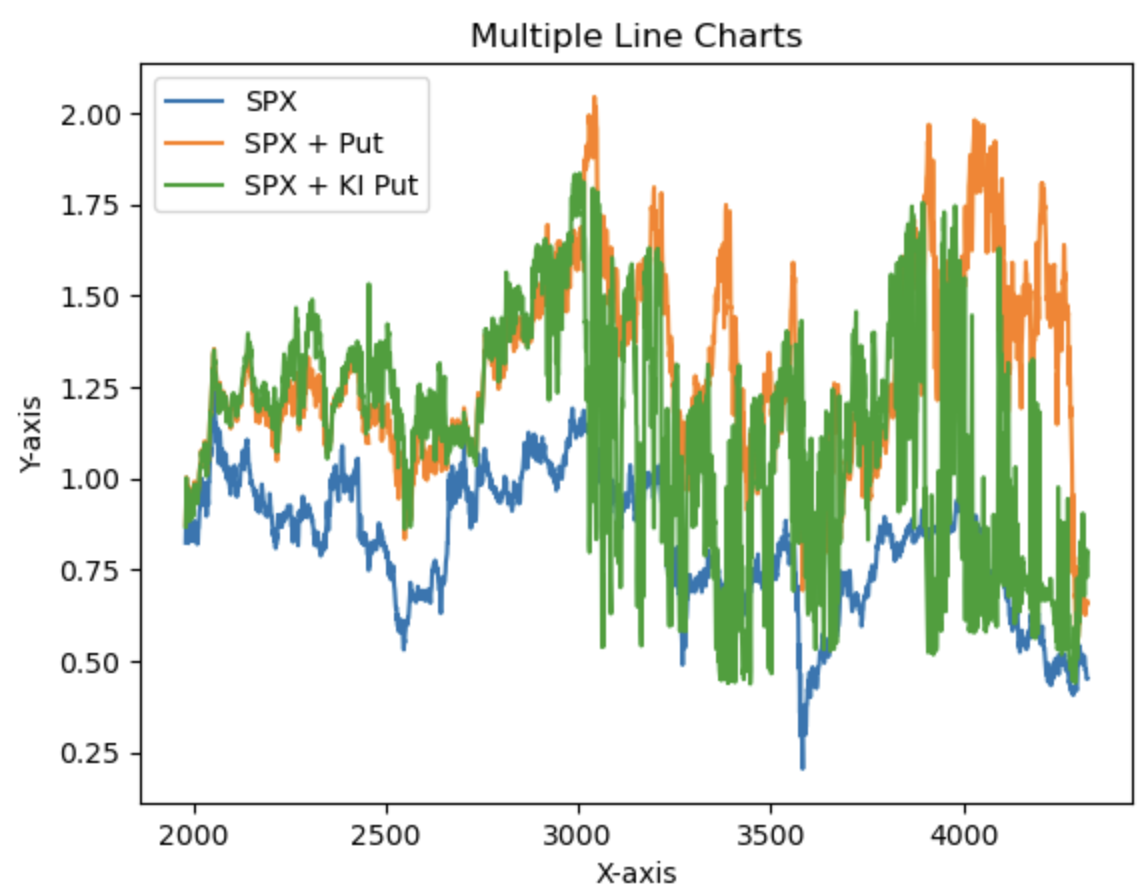
\includegraphics[width=10cm]{5Yrolling.png}
    \caption{Sharpe ratio of strategies using 5Y rolling window}
    \label{fig:galaxy}
\end{figure}

\qquad Core metrics are pointed in the table below. As we can see, vanilla put strategy has lower max drawdown. However, average return is higher using knock-in put strategy. \\

\begin{tabularx}{0.95\textwidth} { 
  | >{\raggedright\arraybackslash}X
  | >{\raggedright\arraybackslash}X 
  | >{\raggedright\arraybackslash}X
  | >{\raggedright\arraybackslash}X |
 }
 \hline
 \textbf{Parameter} & \textbf{SPX} & \textbf{SPX + Put}  & \textbf{SPX + KI Put}  \\
 \hline
 \textbf{Sharpe Ratio} & 0.8246  & 1.2973 & 1.1180  \\
 \hline
 \textbf{Average Return} & 14.33\%  & 13.95\% & 15.54\%  \\
 \hline
 \textbf{Max Draw Down} & 22.21\% & 12.15\% & 18.36\%  \\
 \hline
\end{tabularx}
\\

\qquad Figures 10\&11 below show visually, how strategies behave during different market regimes.

\begin{figure}[!tbp]
\centering
  \begin{minipage}[b]{0.45\textwidth}
    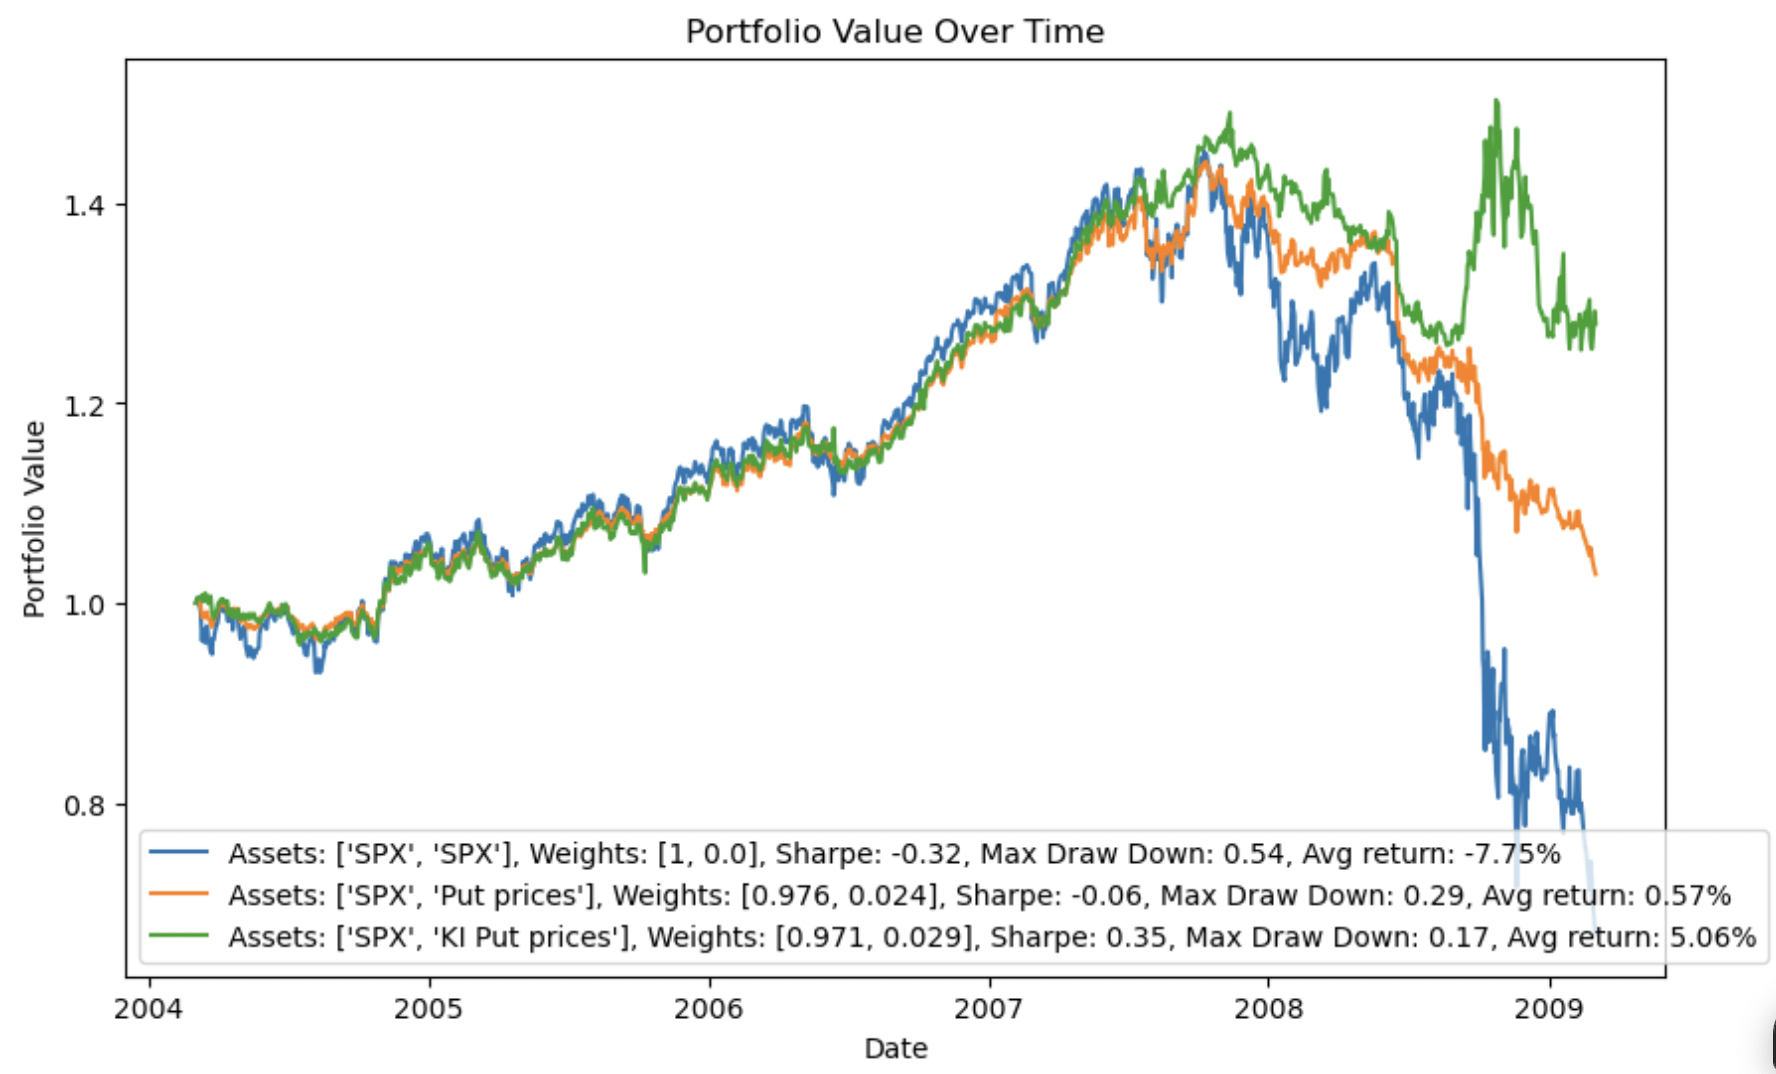
\includegraphics[width=\textwidth]{5yearfalling.png}
    \caption{5 year period of falling market}
  \end{minipage}
  \hfill
  \begin{minipage}[b]{0.45\textwidth}
    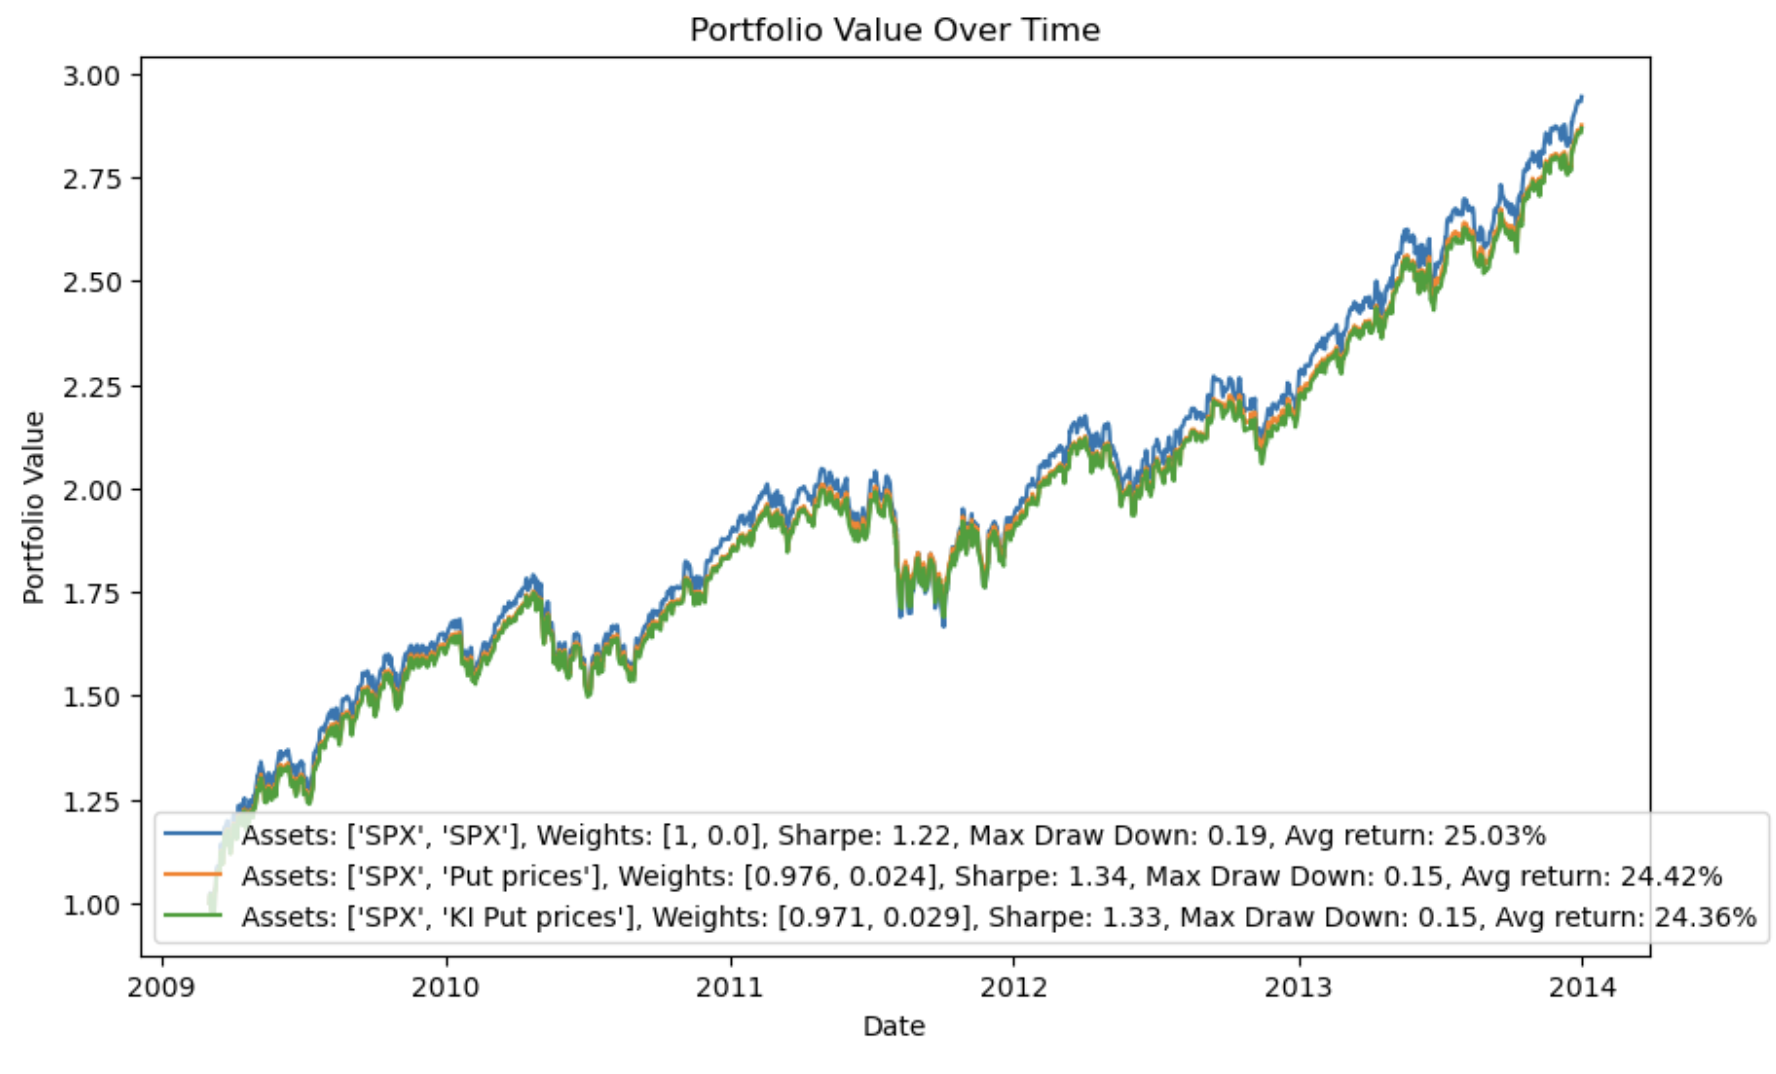
\includegraphics[width=\textwidth]{5Ygrowing.png}
    \caption{5 year period of growing market}
  \end{minipage}
\end{figure}

\qquad Finally, we can conclude, that hedging strategies improves basic metrics compared to long only strategies. Moreover, impact on average return can be insignificant. Knock in put options can be used as an efficient alternative to vanilla put options and in general show comparable or better results.

\section{Potential improvements}
\subsection{Knock-In Put Strategy}
\qquad This paper proves, that using exotic options in hedging can be beneficial for investors. However, the following improvements and research can be done:
\begin{itemize}
\item Value of the barrier in this paper was found empirical way, by testing various options. Further it can be found using more advanced optimization metrics such as gradient descent.
\item Other types of options can be tested for the efficiency. Potentially, digital options can be used for hedging as well. 
\end{itemize}

\subsection{Simulation}
We implemented the strategies on this paper based on historical data. Thus, there is confirmation bias where our results are dependent to the realization of past data. In other words, we fine-tune the strategies in such a way that they best fit the data. 

In order to achieve more robust results we need to implement Monte Carlo simulation. For example, the S\&P500 data could be divided into consecutive buckets (e.g. 5 years). We could calculate the drift and diffusion term for each bucket. Next, we would get the correlation of the S\&P500 with the rest of time series such as the Treasury rates and the VIX. This way, we could use Cholesky decomposition to maintain the structure of the stochastic dynamics while allowing for simulation.  

\subsection{Metrics}
As mention in the Metrics section, a possible area of improvement revolves around exploring more metrics such as the expected shortfall (Homescu, 2014) and parametric-VaR (Bhansali, 2014).

\section{Conclusion}

\qquad Based on the empirical testing of various approaches, including an active put protective monetization strategy by Bhansali [2020], a European knock-in put option strategy, and volatility index option strategies, we can arrive at the following  conclusion:

The conducted analysis and comparison of the three approaches, considering Sharpe ratio, drawdown, and net returns over a 21-year period, have provided valuable insights into their respective performances. The results indicate that both the active put protective monetization strategy and the European knock-in put option strategy outperform volatility-index hedging (e.g., VIX calls) in terms of risk-adjusted returns.

However, it is worth noting that the superior performance of active monetization and European knock-in options comes with the potential drawback of liquidity constraints and transaction costs, which are often challenging to quantify accurately. Despite these challenges, a well-monitored active monetization strategy has demonstrated its ability not only to hedge the downside of a portfolio but also to function as an offensive tail-risk hedging strategy in the medium-term. This versatility in risk management further strengthens the appeal of such strategies for investors seeking to protect and enhance their portfolios.

The empirical evidence presented in this project showcases the potential of both active monetization and European knock-in options, with supporting figures to substantiate their effectiveness. However, it is worth investigating further into the liquidity aspect of knock-in options, as they might exhibit limitations in this regard. Future research can explore backtesting knock-in options with over-the-counter (OTC) data to ascertain the feasibility of implementing frequent trades using this strategy.

Notably, active monetization strategies have demonstrated simplicity and ease of implementation, particularly in the case of a SP500 portfolio, where the empirical analysis suggests a 5x 50\% allocation rule can lead to improved overall performance, especially in the right-tail scenarios.

In conclusion, this study has provided valuable insights into the performance of various risk management strategies, and it supports the notion that active put protective monetization and European knock-in put options offer superior results compared to volatility-index hedging. Nevertheless, investors must carefully consider liquidity constraints and transaction costs associated with these strategies. Additionally, future research efforts should focus on exploring OTC data for knock-in options to evaluate their practicality in frequent trading scenarios. Furthermore, it is essential to tailor active monetization rules according to specific use-cases, as they have the potential to not only hedge downside risk but also enhance overall portfolio performance, especially in favorable market conditions.

\section{Appendix}

In order to showcase our results, we designed a Plotly and Dash dashboard. Here, we decided to implement the three core strategies involving vanilla put options. This way, the user can get a better understanding on how they compare with each other. 

As shown in the dashboard, the user has the option to select the dates for the backtest of each strategy:

\begin{itemize}
\item \textbf{Buy and Hold:} Buy and hold the underlying, allowing the user to select the initial value of the portfolio.
\item \textbf{Put Until Expiration:} Buy the underlying and the put option, allowing the user to select the initial value of the portfolio and the percentage allocation of puts.
\item \textbf{Put Monetization Strategy:} Buy the underlying and the put option with early monetization based on Bhansali, allowing the user to select the initial value of the portfolio, the percentage allocation of puts, and the multiplier.
\end{itemize}

While the dashboard only displays a subsection of the full set of strategies implemented throughout the paper, it gives a dynamic interaction to the reader for a richer understanding.

\begin{figure}[htp]
    \centering
    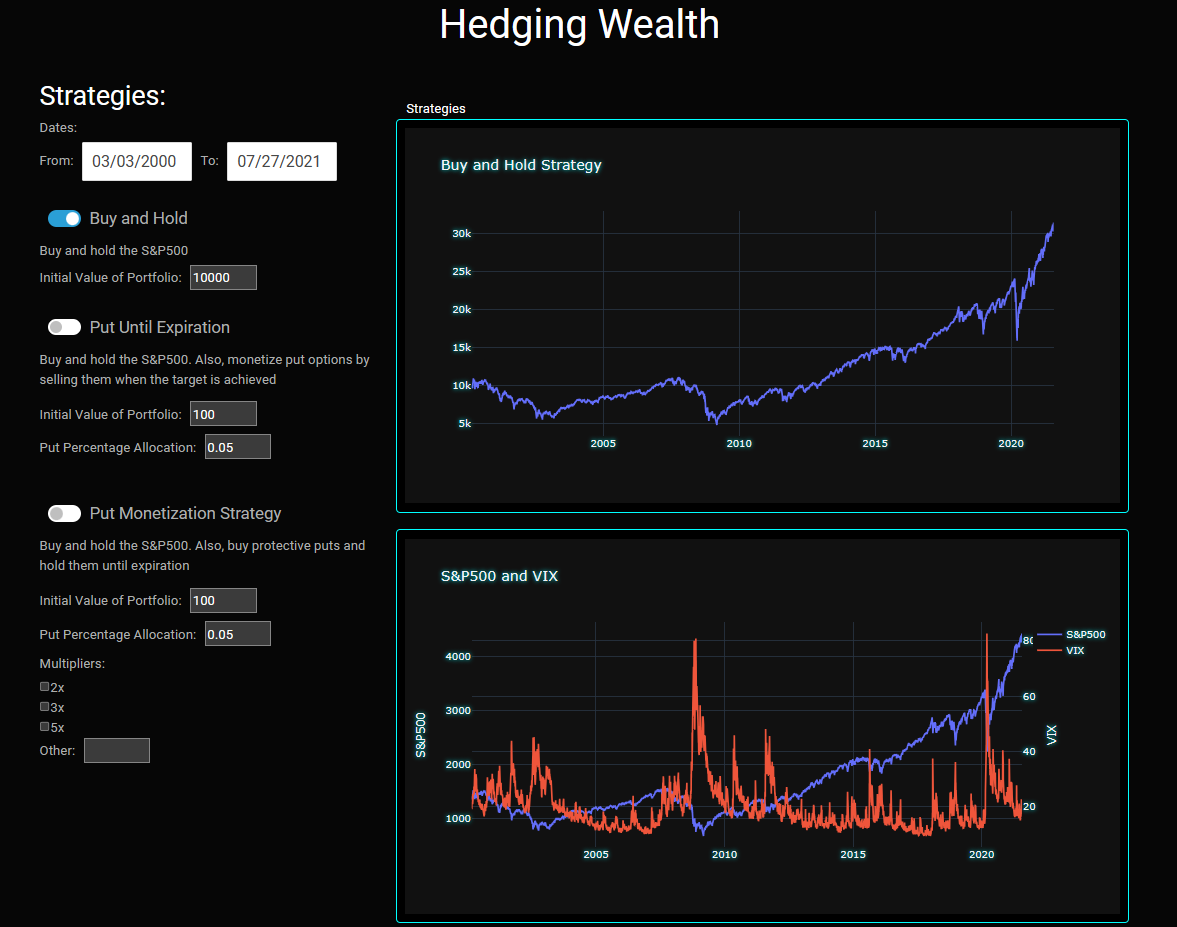
\includegraphics[width=13cm, height=8cm]{Hedging_wealth.png}
    \caption{Dashboard}
    \label{fig:galaxy}
\end{figure}

\newpage

\pagebreak

\section{References}
\begin{itemize}
\item Bhansali, Vineer. Tail risk hedging: Creating robust portfolios for volatile markets. McGraw Hill Professional, 2013.
\item Bhansali, Vineer. "Tail-Risk Management for Retirement Investments." The Journal of Retirement 2.3 (2015): 78.
\item Bhansali, Vineer. "Right Tail Hedging: Managing Risk When Markets Melt Up." The Journal of Portfolio Management 44.7 (2018): 55-62.
\item Bhansali, Vineer, et al. "Monetization Matters: Active Tail Risk Management and the Great Virus Crisis." The Journal of Portfolio Management 47.1 (2020): 16-28.
\item Israelov, Roni, and Lars N. Nielsen. "Still not cheap: Portfolio protection in calm markets." The Journal of Portfolio Management 41.4 (2015): 108-120.
\item Koekebakker, Steen, and Valeriy Zakamulin. "Warren Buffett versus Zvi Bodie: Should You Buy Or Sell Put Options?." The Journal of Wealth Management 24.2 (2021): 65-81.
\printbibliography
\end{itemize}

\end{document}
